\documentclass[xcolor=pdftex,dvipsnames,table,mathserif,aspectratio=169]{beamer}
\usetheme{metropolis}
%\usepackage{times}
%\usefonttheme{structurebold}

\usepackage[english]{babel}
%\usepackage[table]{xcolor}
\usepackage{pgf,pgfarrows,pgfnodes,pgfautomata,pgfheaps}
\usepackage{amsmath,amssymb,setspace,centernot}
\usepackage[latin1]{inputenc}
\usepackage[T1]{fontenc}
\usepackage{relsize}
\usepackage{pdfpages}
\usepackage[absolute,overlay]{textpos} 


\newenvironment{reference}[2]{% 
  \begin{textblock*}{\textwidth}(#1,#2) 
      \footnotesize\it\bgroup\color{red!50!black}}{\egroup\end{textblock*}} 

\DeclareMathSizes{10}{10}{6}{6} 

\begin{document}
\title{Part 6: Model Selection and Intro to ML}
\author{Chris Conlon}
\institute{Applied Econometrics II}
\date{\today}

\frame{\titlepage}
\section{Principal Components Regression}

\begin{frame}
\frametitle{Other Data Reduction Techniques}
We have other data reduction techniques with a long history in Econometrics
\begin{itemize}
\item Principal Components
\item Factor Analysis
\item Partial Least Squares
\end{itemize}
\end{frame}

\begin{frame}
\frametitle{Principal Components}
Suppose we have a very high dimensional $X$ where we have a high degree of correlation among the components $x_j$. 
\begin{itemize}
\item We can start by computing the appropriate correlation matrix $C=E[\tilde{X}'\tilde{X}]$ where $\tilde{X}$ denotes we have standardized each column $x_j$ to have mean zero and variance 1.
\item Diagonlize $C$ via the eigen-decomposition $V^{-1} C V = D$ where $D$ is the diagonal matrix of eigenvalues.
\item Sort $D$ and the corresponding columns of $V$ in decreasing order of the eigenvalues $d_j$.
\item Choose a subset of $m < K$ eigenvalues and eigenvectors and call that $V_m$ and $\lambda_m$
\item Compute transformed data: $Z_m = V_m \tilde{X}$ which is of dimension $N \times m$ instead of $N \times K$.
\end{itemize}
\end{frame}

\begin{frame}
\frametitle{Principal Components}
\begin{itemize}
\item If $m \ll K$ then we can substantially reduce the dimension of the data.
\item The idea is to choose $m$ so that $(Z'Z)$ spans approximately the same space that $(X'X)$ does.
\item This works because we use the \alert{principal eigenvectors} (those with the largest eigenvalues).
\item The first eigenvector explains most of the variation in the data, the second the most of the remaining variation, and so on.
\item You may also recall that eigenvectors form an \alert{orthonormal basis}, so each dimension is linearly independent of the others.
\item As eigenvalues decline, it means they explain less of the variance.
\end{itemize}
\end{frame}

\begin{frame}
\frametitle{Principal Components}
Output from software will inlcude
\begin{itemize}
\item Coefficients: these transform from $X\rightarrow Z$
\item Score: these are the transformed $Z$'s
\item Latent/Eigenvalue: the corresponding Eigenvalue
\item Explained/Cumulative: cumulative explained variance $ \sum_{j=1}^m( \lambda_j / \sum_k \lambda_k)$
\item Stata: \texttt{pca}, Matlab: \texttt{pca}, R/stats: \texttt{princomp}.
\end{itemize}
\end{frame}

\begin{frame}
\frametitle{Principal Components}
How many components?
\begin{itemize}
\item Choose \# of components by the eigenvalues or \% of variance explained
\item Common cutoffs are 90-95\% of variance.
\item Eigenvalue based cutoff rules (only take eigenvalues $ > 1$).
\item Most common method is to eyeball the scree plot.
\end{itemize}
\end{frame}


\begin{frame}
\frametitle{Principal Components}
\begin{center}
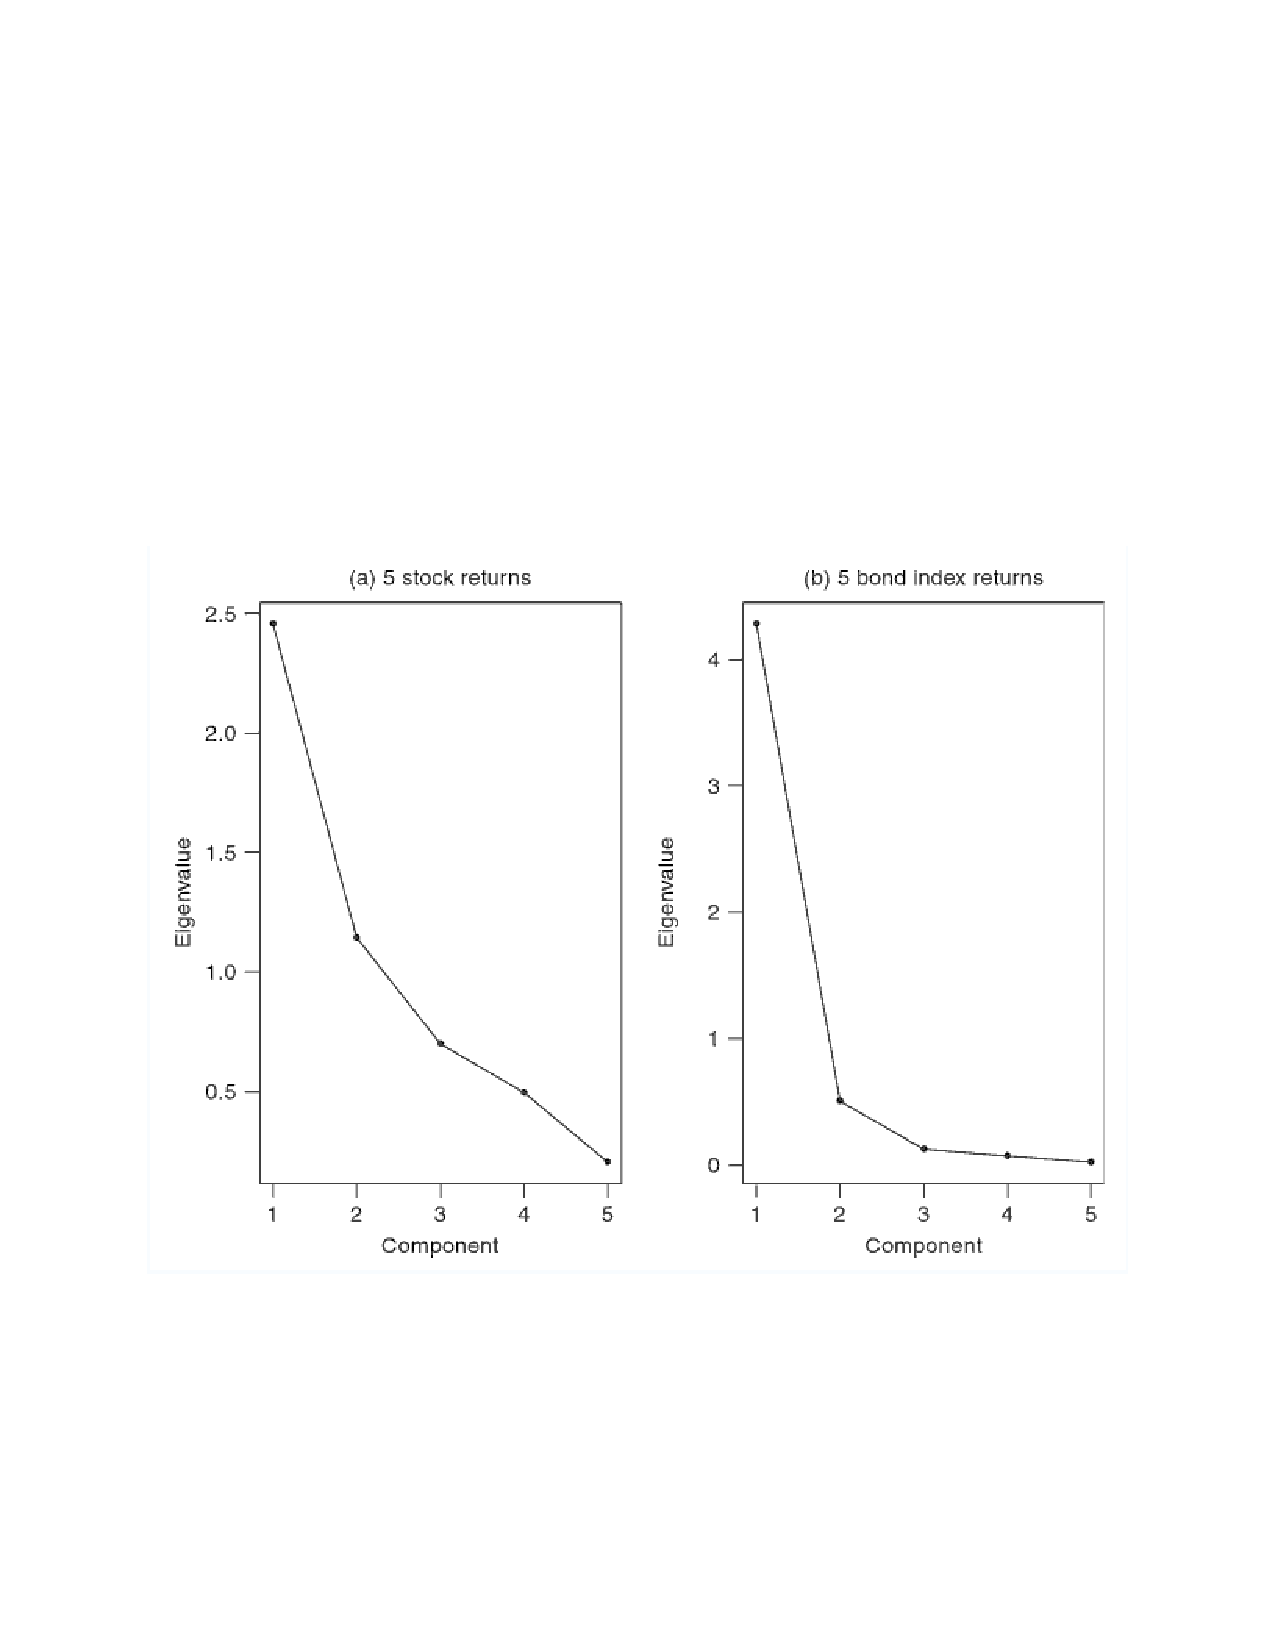
\includegraphics[height=0.9\textheight]{./resources/princomp1}
\end{center}
\end{frame}

\begin{frame}
\frametitle{Principal Components}
\begin{center}
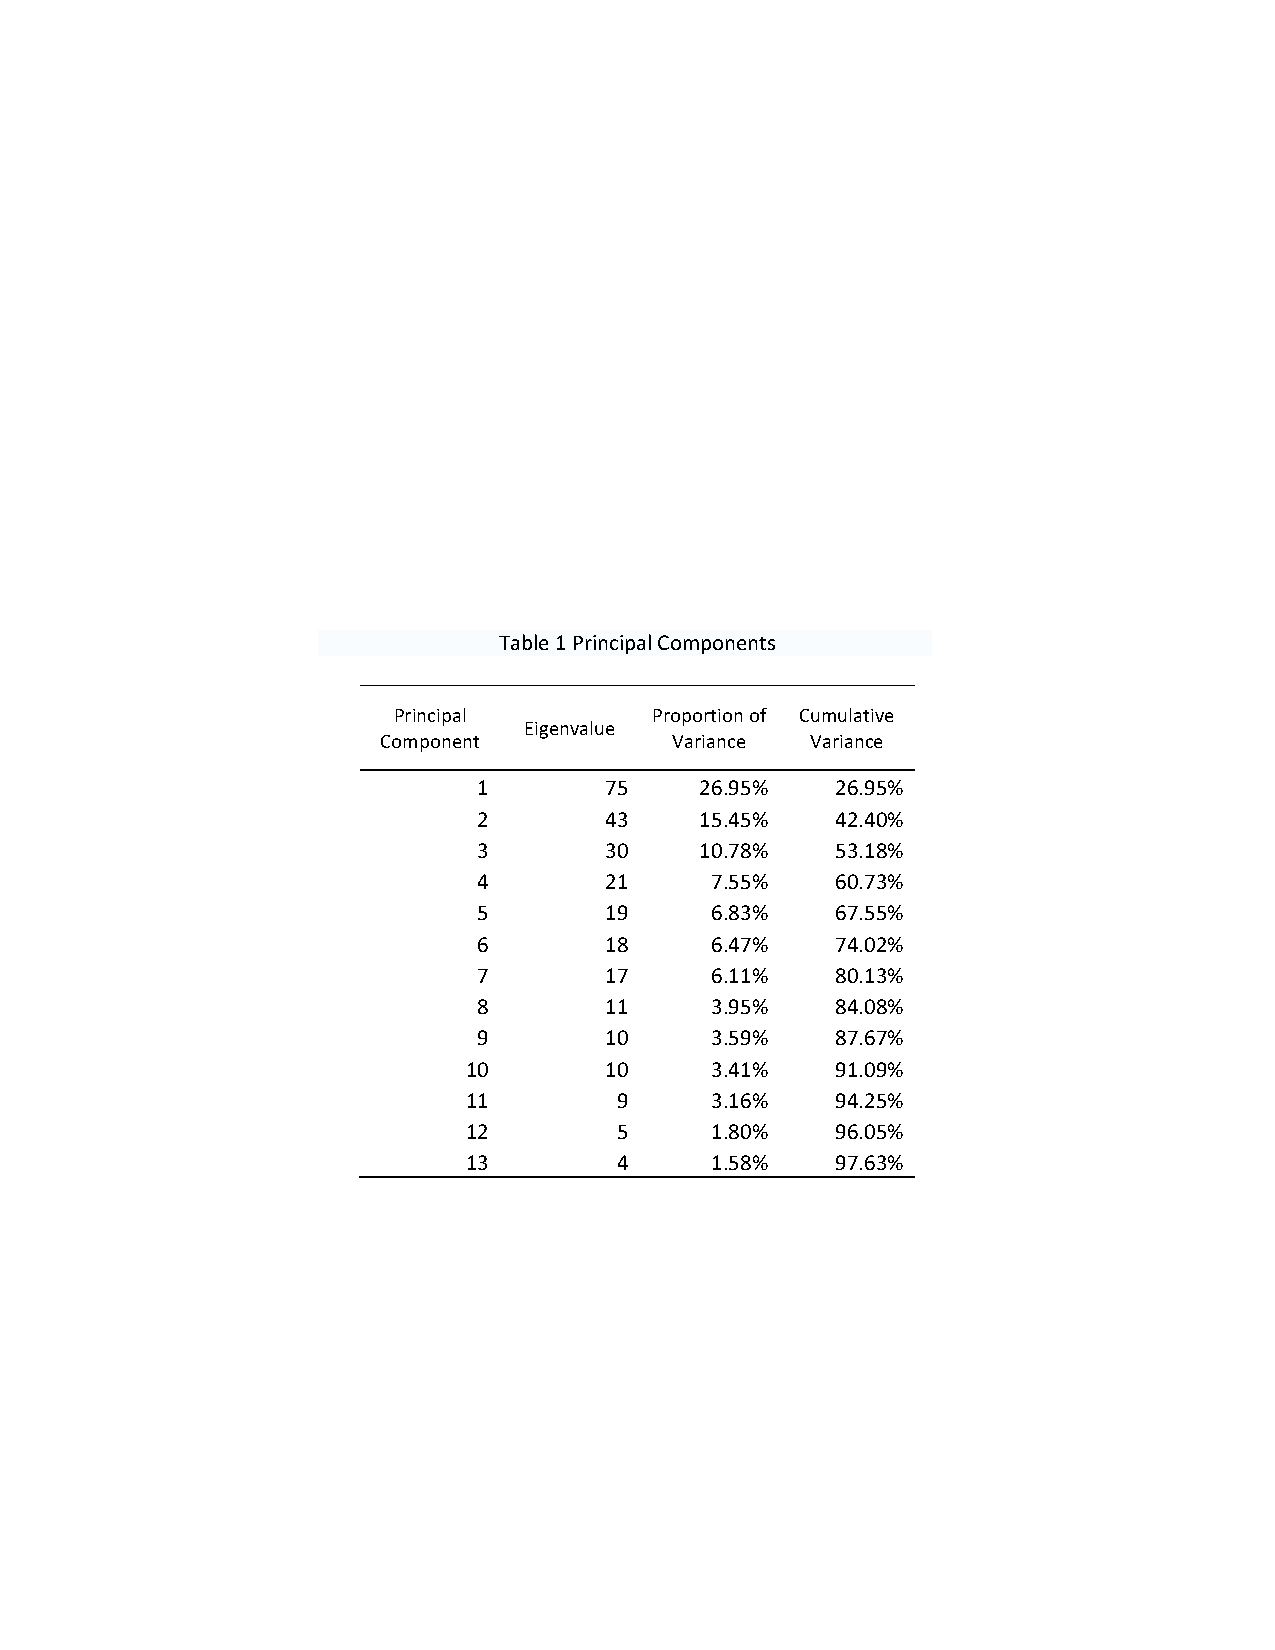
\includegraphics[height=0.9\textheight]{./resources/princomp2}
\end{center}
\end{frame}

\begin{frame}
\frametitle{Principal Components}
\begin{itemize}
\item We can run a regression on principal components $Z$'s and then recover the betas of the $X$'s
\begin{eqnarray*}
\hat{y}_{(M)}^{pcr} = \overline{y} \mathbf{1} + \sum_{m=1}^M \hat{\theta}_m \mathbf{z}_m
\end{eqnarray*}
\item Because principal components are orthogonal we can find coefficients using univariate regression $\hat{\theta}_m = \langle \mathbf{z_m} , \mathbf{y} \rangle / \langle \mathbf{z_m} , \mathbf{z_m} \rangle$.
\item We can recover the $x$ coefficients because the PCA is a linear transformation:
\begin{eqnarray*}
\hat{\beta}^{PCR} = \sum_{m=1}^M \hat{\theta}_m v_m
\end{eqnarray*}
\end{itemize}
\end{frame}

\begin{frame}{Principal Components (and Ridge)}
\begin{itemize}
\item If $M=P$ (we use all components) then PCR = OLS.
\item If $M < P$ then we discard the $p-M$ smallest eigenvalue components
\item This is similar to ridge which shrinks $\beta$'s for components with small eigenvalues.
\item Think about the variance matrix $X'X/n$ or $X' X = V D^2 V'$.
\item First component (largest eigenvalue) is $\mathbf{z_1} = \mathbf{X} v_1 = \mathbf{u_1} d_1$.
\item Variance is $Var(\mathbf{z_1}) = Var (\mathbf{X} v_1) = \frac{d_1^2}{N}$ ($\mathbf{z_1}$ is first principal component of $\mathbf{X}$).
\end{itemize}
\end{frame}



\begin{frame}
\frametitle{Principal Components}
\begin{center}
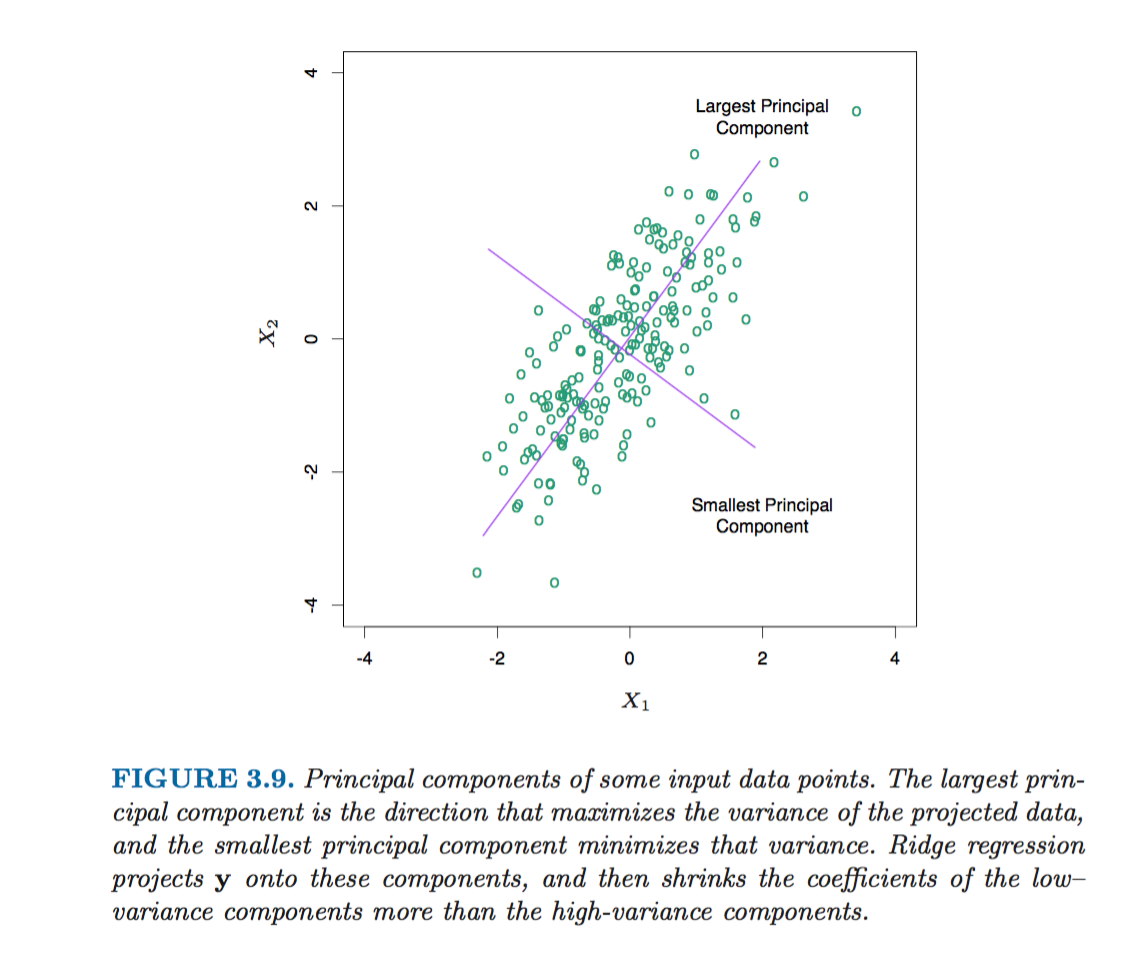
\includegraphics[height=0.9\textheight]{./resources/princompfig}
\end{center}
\end{frame}




\begin{frame}
\frametitle{Principal Components And Ridge}
Consider the objective function that Ridge minimizes:
\begin{eqnarray*}
RSS(\lambda) = (\mathbf{y} - \mathbf{X} \beta)'  (\mathbf{y} - \mathbf{X} \beta)' + \lambda \beta' \beta
\end{eqnarray*}
And the solution (which addresses multicolinearity!)
\begin{eqnarray*}
\hat{\beta}_{ridge} = (\mathbf{X}' \mathbf{X} + \lambda \mathbf{I})^{-1} \mathbf{X}' \mathbf{y}
\end{eqnarray*}

\end{frame}

\begin{frame}
\frametitle{Principal Components And Ridge}
Just like we can diagonalize (some) square matrices, we can take the \alert{singular value decomposition} (SVD) of any matrix $\mathbf{X}$ that is $N \times p$
\begin{eqnarray*}
\mathbf{X}=\mathbf{U} \mathbf{D} \mathbf{V}'
\end{eqnarray*}
\begin{itemize}
\item $\mathbf{U}, \mathbf{V}$ are $N \times p$ and $p \times p$ orthonormal matrices ($\mathbf{U}$ spans the column space, and $\mathbf{V}$ spans the row space of $X$.)
\item $\mathbf{D}$ is a diagonal matrix $p \times p$ with elements corresponding to the singular values of $\mathbf{X}$.
\item If $\mathbf{X}$ is a square, diagonalizable matrix the singular values are equal to the eigenvalues.
\end{itemize}
\end{frame}

\begin{frame}
\frametitle{Principal Components And Ridge}
Now the least squares solution is simple
\begin{align*}
\mathbf{X} \hat{\beta}^{ols} = \mathbf{X} (\mathbf{X}'\mathbf{X})^{-1} \mathbf{X}' \mathbf{y} = U U' \mathbf{y}.
\end{align*}
\begin{itemize}
\item $\mathbf{U}' \mathbf{y}$ are the values of $\mathbf{y}$ mapped into the orthonormal basis $\mathbf{U}$.
\item This looks a lot like $\mathbf{QR}$ except that we have chosen a different basis.
\end{itemize}
Ridge is simple too:
\begin{align*}
\mathbf{X} \hat{\beta}^{ridge} = \mathbf{X} (\mathbf{X}'\mathbf{X} + \lambda \mathbf{I})^{-1} \mathbf{X}' \mathbf{y} &= \mathbf{U D} (\mathbf{D}^2 + \lambda \mathbf{I})^{-1} \mathbf{D} \mathbf{U}' \mathbf{y}\\
&= \sum_{j=1}^p \mathbf{u}_j  \frac{d_j^2}{d_j^2 + \lambda} \mathbf{u}_j' \mathbf{y}
\end{align*}
\begin{itemize}
\item Same change of basis. Now we shrink each component by $d_j^2/(d_j^2 + \lambda)$.
\end{itemize}
\end{frame}



\begin{frame}
\frametitle{Principal Components}
\begin{center}
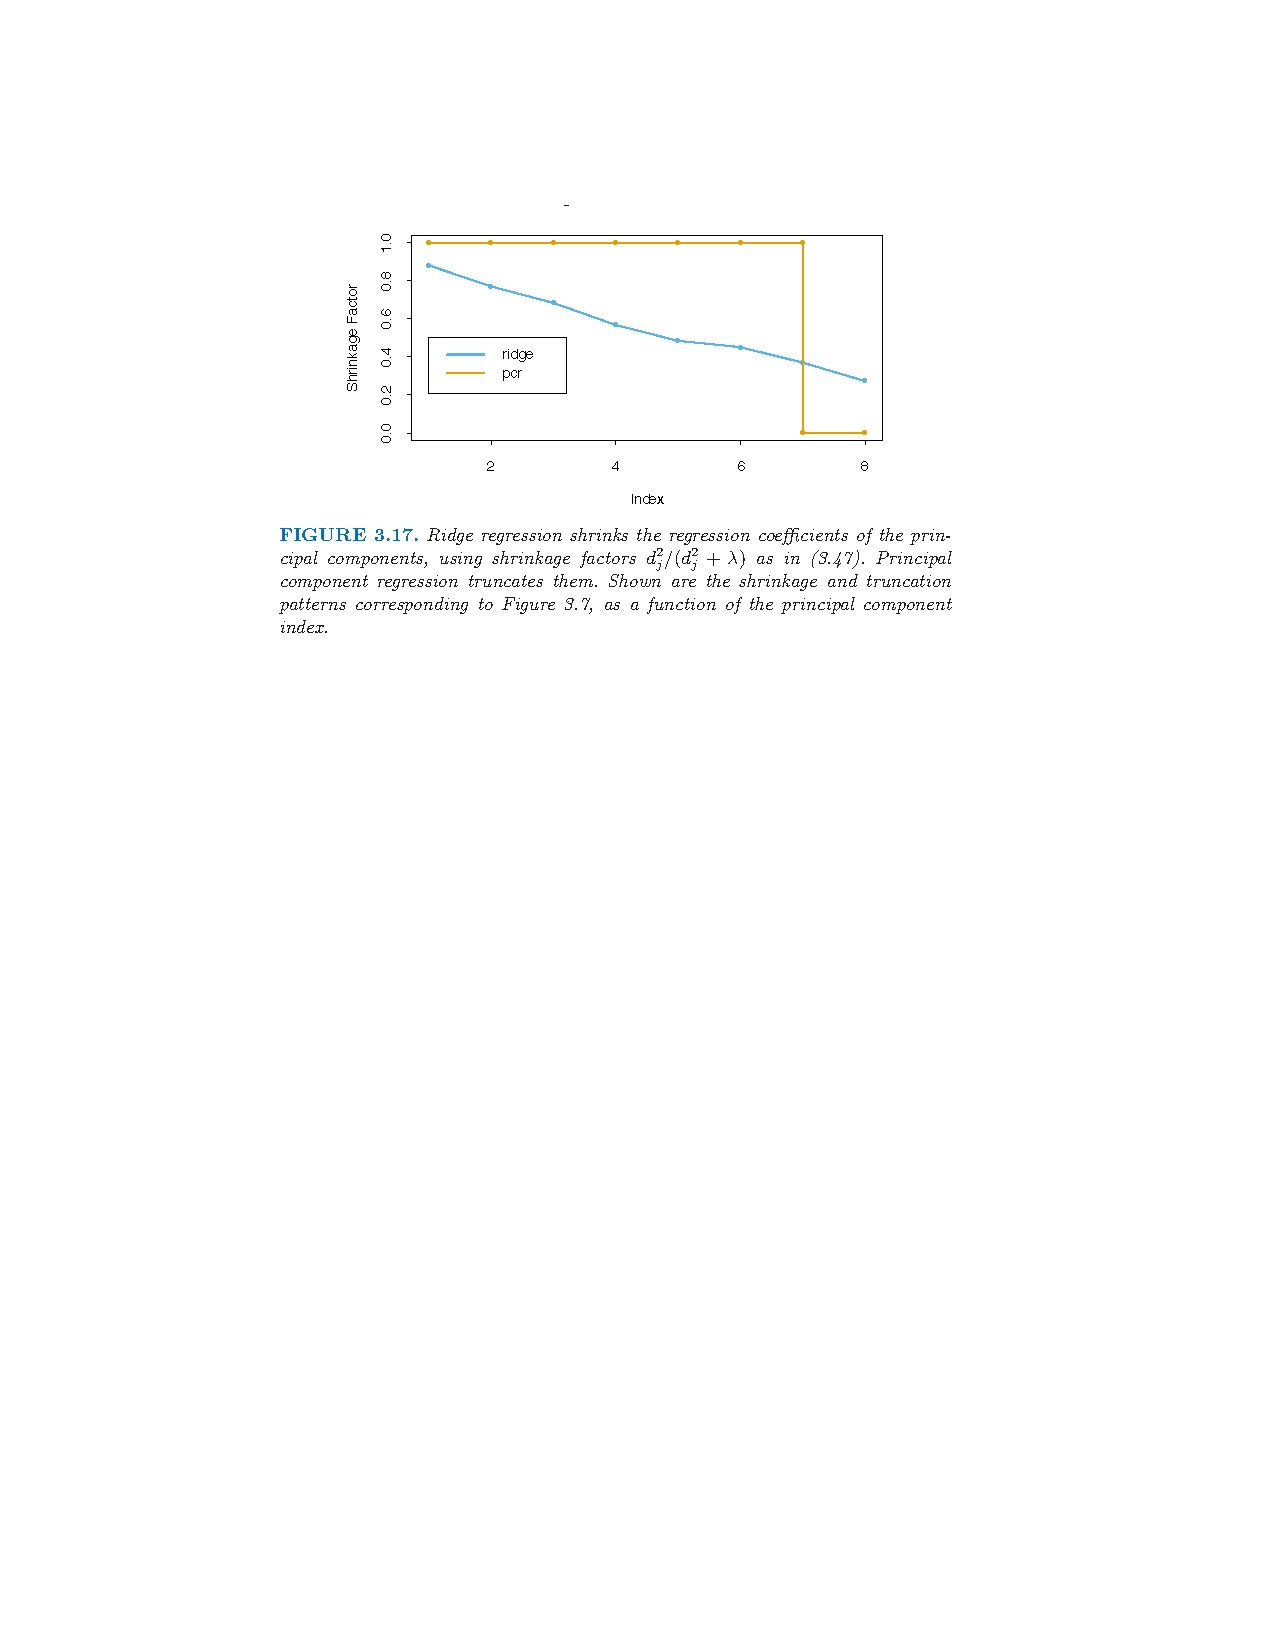
\includegraphics[height=0.85\textheight]{./resources/pcrridge}
\end{center}
\end{frame}


%
%\begin{frame}
%\frametitle{Hansen Singleton (1982)}
%\begin{itemize}
%\item This is the original GMM example, though it comes from macro-finance not microeconometrics
%\begin{eqnarray*}
%\max_{c_{t+i},A_{t+i}}&& E_t \sum_{i=0}^{\infty} \frac{U(c_{t+i})}{(1+\delta)^i} \quad \mbox{subject to } \\
%A_{t+i} &=& (1+r) A_{t+i-1} + y_{t+i} - c_{t+1} \\
%0&=&\lim_{i \rightarrow \infty} E_t A_{t+i} (1+r)^{-i} 
%\end{eqnarray*}
%\item $A_t$ are your investment assets with return $r$ and discount factor $\delta$
%\item $y_t$ is your income in period $t$, $c_t$ is your consumption 
%\end{itemize}
%\end{frame}
%
%\begin{frame}
%\frametitle{Hansen Singleton (1982)}
%\begin{itemize}
%\item Assume CRRA utility with risk aversion $\gamma$
%\begin{eqnarray*}
%U(c_{t+i})  = \frac{c_{t+i}^{1-\gamma}}{1-\gamma}
%\end{eqnarray*}
%\item We can take the first-order/Euler conditions and get:
%\begin{eqnarray*}
%E_t \left(\underbrace{\frac{1+r}{1+\delta} c_{t+1}^{-\gamma} - c_{t}^{-\gamma}}_{g(x_{t+i},\theta)}\right) = 0
%\end{eqnarray*}
%\item We want to estimate the ``deep parameters'' $\theta \equiv (\gamma,\delta)$.
%\end{itemize}
%\end{frame}
%
%\begin{frame}
%\frametitle{Hansen Singleton (1982)}
%\begin{itemize}
%\item We can solve for $\theta$ without actually solving the dynamic programming problem!
%\item We just need some instruments $z_t$ that are conditionally independent/orthogonal to $g(x_{t+i},\theta)$ so that
%\begin{eqnarray*}
%E_t [g(x_{t+i},\theta) | z_t] = 0 \Rightarrow E_t [g(x_{t+i},\theta)  z_t] = 0 
%\end{eqnarray*}
%\item This is \alert{nonlinear GMM}. We need a matrix of instruments $z_t$ with dimension $N \times Q$ where $Q \geq \dim(\theta)$.
%\item Where do we get $z_t$? $\rightarrow$ Economic Theory!
%\end{itemize}
%\end{frame}
%
%
%\begin{frame}
%\frametitle{Hansen Singleton (1982)}
%Consider $E_t [g(x_{t+i},\theta) | z_t] = 0$.
%\begin{itemize}
%\item The error arises from the error in the Euler equation: deviations between observed behavior and expected behavior.
%\item If the model is true this optimization error should be independent of anything known to the agent at the time the decision was made.
%\item We often write: $E_t [g(x_{t+i},\theta) | z_t, \Omega_t] = 0$ where $\Omega_t$ is everything known by the agent up until time $t$ (including the full history).
%\item If we have some potential instrument $z_t$ and use the full history then $z_{t-1},z_{t-2},\ldots$ are all valid instruments
%\item If we use the conditional moment restriction $E_t [g(x_{t+i},\theta) | z_t, \Omega_t] = 0$ then any nonlinear function of $z_t$ is also an instrument
%\begin{eqnarray*}
%E_t [g(x_{t+i},\theta) f(z_{t,t-1,\ldots,0}) ]  = 0
%\end{eqnarray*}
%\end{itemize}
%\end{frame}
%
%
%\begin{frame}
%\frametitle{Hansen Singleton (1982)}
%\begin{itemize}
%\item We have literally infinite possibilities to construct instruments $z_t, z_t^2, z_t^3, z_t \cdot z_{t-1}, \ldots$
%\item But our instruments could be \alert{weak} even though we have many of them.
%\item And they might be highly correlated with each other.
%\item Carrasco (2012) suggests \alert{regularization} on the instruments first.
%\item One possibility for $f(z_{t},z_{t-1},z_{t-2},\ldots)$ is to take several higher order interactions and take the first $Q$ principal components.
%\item Even though we might have 100 instruments, after running PCA we might find that 99\% of our variation is only in 6 components. In that case we should not try and identify more than 6 parameters!
%\item Conlon (2014) suggests this as a test of non-identification in nonlinear BLP-type GMM problems.
%\end{itemize}
%\end{frame}

\begin{frame}
\small
\frametitle{Factor Models}
\begin{itemize}
\item Related to PCA is the \alert{factor model}
\item These are frequently used in finance for asset pricing. 
\begin{eqnarray*}
r_i = b_0 + b_1 f_1 + b_2 f_2 + \ldots b_p f_p + e_i
\end{eqnarray*}
\item Typically we choose factors so that $E[f_i] = 0$ and $E[f_i e_i] = 0$ and that $Cov(f_i,f_j) = 0$ for $i \neq j$.
\item That is we choose scaled factors to form an orthogonal basis (which makes pricing assets easier).
\item Instead of choosing $f$ to best explain $X'X$ we choose it to best explain $r$ by taking linear combinations of our $X$'s.
\item CAPM is a single factor model (where the factor is the \alert{market return}).
\item Fama-French have expanded to a 5 factor model (book-to-market, market-cap, profitability, momentum)
\item Ross's APT is another form of a factor model.
\end{itemize}
\end{frame}

\begin{frame}
\frametitle{Factor Models: Other Examples}
\small
\begin{itemize}
\item \textit{Eigenfaces} reduces your face to the first few eigenvalues -- this is how face detection works!
\item In psychometrics they use data from multiple tests to measure different forms of intelligence (mathematical reasoning, verbal, logical, spatial, etc.)
\begin{itemize}
\item An old literature searched for general intelligence factor $g$
\item Nobody can tell what the GMAT measured!
\end{itemize}
\item In marketing PCA/factor analyses are used in the construction of \textit{perceptual maps}
\item Marketing practitioners use FA/PCA more than academics these days (guess: maybe?)
\end{itemize}
\end{frame}



\end{document}
